\documentclass[11pt]{article}
\usepackage[utf8]{inputenc}
\usepackage{setspace} \doublespacing
\usepackage{graphicx}
\pagenumbering{roman} 
\parskip 0.05in
\parindent 0.2in
\title{\vspace{-3cm}{\textbf{Title IX Compliance and Equity in Athletics\\{STAT 3493W}}}}
\author{Nidhi Jayakumar Nair}

\begin{document}
       
\maketitle

\section{Abstract}

June 23rd, 2022 marked the 50th anniversary of Title IX laws, the historic federal civil rights law that has been credited with profoundly changing education by gender in the United States. Title IX compliance in college-level athletics is a contentious issue as budget cuts due to the COVID-19 pandemic in 2021 forced universities to reevaluate their allotments to club sports helmed by female players. One of the ways in which Title IX compliance is measured in universities is by showing that the school is fully and effectively meeting its students' interests and abilities to participate in sports by gender and athletic expenditure. This paper seeks to use the Integrated Postsecondary Education Data System (IPEDS) and the Equity in Athletics Disclosure (EADA) datasets to study Title IX compliance at the University of Connecticut and all eleven Big East schools.

\section{Keywords}
Title IX, discrimination, sports, athletics, civil rights

\section{Introduction}

The passing of two landmark laws in 1964 set the foundation for Title IX, the historic gender equity law that outlaws discrimination based on sex in most American universities. Lack of compliance with Title IX in athletics is a contentious topic in public discourse, especially at the University of Connecticut, when Title IX violations were bought into focus through a prominent lawsuit filed by the UConn rowing team in 2020 \cite{Doyle}. The University was accused of not being compliant with Title IX since 2008 by external court-ordered auditors, thus exhibiting the pertinence of Title IX legislative compliance in advancing civil right discourse.

\medskip

This issue is also important because, despite strong federal laws and increasing female undergraduate enrollment in universities around the country, women lag behind men by all measurable criteria related to sports, including opportunities to play, scholarship dollars, and treatment, and those gaps are growing. Studies have shown that while socialization and negligible evolutionary effects have reduced demonstrated female interest in sports, women have a relatively equal interest and inclination toward athletics and team-based sports \cite{Deaner}.

This mismatch in female athletic interest and institutional services offered by universities at an undergraduate level has resulted in an increase in public focus on Title IX noncompliance, and there has been legal pushback as a result. 

\medskip

Studies on this issue have detailed the specific lawsuits that have resulted from legal actions taken by club sports against universities that are often accused of cutting women's teams during times of financial hardship. For example, in a seminal case, Brust vs. Regents of University of California, Davis, the plaintiffs claimed that the university showed systemic discrimination under Title IX laws by eliminating existing women's varsity athletic teams, cutting scholarships and opportunities for women athletes. Plaintiffs claimed that there was a 6 \% differential between female enrollment and female varsity-level athletics participation, thus pointing to a violation of Title IX laws that require substantial proportionality between undergraduate female enrollment and athletic services. In this case, UC Davis was required to exhibit further evidence that they were in compliance with Title IX laws \cite{Brust}.

\medskip

Data-backed evidence in Title IX litigation is a relatively new approach to civil rights advancement, and this paper will be a unique and new contribution to limited scholarly research on Title IX compliance using gender-based athletic expenditure in the Big East schools (University of Connecticut, Butler University, Creighton University, DePaul University, Georgetown University, Marquette University, Providence College, Seton Hall University, St. John's University-New York and Villanova University). Using data in the EADA dataset that details student athletic aid given to men's and women's teams as well as expenses for both types of athletic teams, and the undergraduate enrollment numbers provided in the IPEDS dataset, this author seeks to show significant differences in athletic funding allocated to men and women based on their undergraduate enrollments.

\section{Specific Aims}

Title IX rests on issues of fairness and equality, and compliance involves two parts: \emph{quantitative} and \emph{qualitative} components. Title IX has three basic requirements regarding athletics that were developed throughout the 1970s, finalized in 1979, clarified in 1996, and supported by the most recent Office of Civil Rights review of the law in 2002 \cite{Watson}). The three areas are financial assistance; effective accommodation of students' interests and abilities; and benefits, opportunities, and treatments \cite{Watson}). The law requires that schools provide women and girls with equal opportunities to participate, meaning schools must provide women with the chance to be in an official sports team, while also having the same educational and financial benefits provided to men. In order to be compliant with Title IX, a school has to comply with a three-prong test \cite{Mak}.

\textbf{Part One}: Substantial Proportionality.\\
This part of the test is satisfied when participation opportunities for men and women are "substantially proportionate" to their respective undergraduate enrollments. 

\textbf{Part Two}: History and Continuing Practice. \\
This part of the test is satisfied when an institution has a history and continuing practice of program expansion that is responsive to the developing interests and abilities of the underrepresented sex (typically female). 

\textbf{Part Three}: Effectively Accommodating Interests and Abilities. \\ This part of the test is satisfied when an institution is meeting the interests and abilities of its female students even where there are disproportionately fewer females than males participating in sports.

The Office of Civil Rights(OCR) calculates compliance with prong one by analyzing enrollment and student-athlete numbers. For example, if women are 52\% of full-time enrollment at a university with almost 800 total athletes, then OCR only measures compliance within 1.5 percentage differences, which means that women's participation in athletics should be between 50.5\% to 53.5\% to comply with Title IX. Any numbers below or above that would count as a lack of compliance with Title IX's prong one \cite{Schwarz}. Prong one, which is the main relevant measure used in this paper, will analyze interest in sports by measuring declines or upticks in female college enrollment over the years and prong three will use a few other qualitative methods of comparison (like institutional athletics surveys disseminated by the university, or physical education electives offered for both sexes).

This paper will use the metrics of total expenses and athletic aid money as variables to primarily measure part one of the three Title IX compliance prongs. A 1996 amendment to Title IX ensured that colleges and universities were now required to disclose funding and participation rates broken down by gender so this paper will avail those resources to test its hypothesis. The primary hypothesis of the paper is that the Big East schools will be non-compliant with the first prong of substantial proportionality, as measured by testing the relationship between provided athletic expenditure compared to the undergraduate population. Ratios of athletic aid money and total expenses compared to male and female undergraduate enrollment will be compiled, and the ratios will be charted over the course of five years (2015 - 2020). 

This paper also uses the Big East schools because these are NCAA Division I schools which are primarily located in the Northeast and Midwest metropolitan areas \cite{Augustyn}. They are similar in terms of athletic prowess and have won NCAA national championships in men's basketball, women's cross country, field hockey, men's lacrosse, and men's soccer. It is predicted that these schools will have a significant difference in athletic expenses by gender over the past five years, depending on the initial assumption that male and female undergraduates are expected to exhibit a similar interest in team-based athletics.

\section{Data Description}

The IPEDS dataset contains data on male and female undergraduate enrollment in all the Big East schools for the past 30 years \citet{keyi}. The EADA dataset contains extensive data on pay differentials between male and female coach salaries, athletic student aid, and recruiting expenses for male and female teams \citet{keye}. Both datasets have been commissioned by the U.S. Department of Education to provide rapid, customized reports for public inquiries. The EADA dataset is also administered by the Office of Postsecondary Education to provide equity in athletics data. 

The schools under consideration are the Big East schools, which include Butler University, UConn, Creighton University, DePaul University, Georgetown University, Marquette University, Providence College, St. John's University, Seton Hall University, Villanova University, and Xavier University. 

Title IX compliance rests on three prongs, however, this author shall only use the first and third prongs to analyze trends in Title IX compliance (substantial proportionality and effective accommodation of interests). There is no dataset used to measure the first prong, however, the two datasets used by the author allow for the creation of a variable that details an average expenditure: enrollment values for all eleven schools. The third prong will be analyzed by studying a potential mismatch in  rates of undergraduate enrollment compared to athletic services offered by the institutions. 

For the purposes of this paper, the author uses four variables from the EADA dataset: 1) Male Athletic Aid Spending, 3) Female Athletic Aid Spending, 3) Male Team Expenses, 4) Female Team Expenses. From the IPEDS dataset, the author uses two variables: 1) Female Undergraduate Enrollment and 2) Male Undergraduate Enrollment. This data is collected over the course of five years from the fall of 2016 to fall of 2020. Expense: enrollment ratios for male and female athletic teams are calculated by dividing the sum of athletic aid expenditure and total expenses for male and female teams by male and female enrollment. The averages of these ratios for all eleven schools are calculated for each year, and charted over time to analyze trends in athletic expenditure and participation.

\section{Research Methods}

This paper will pull data from the EADA dataset on total expenses and athletic aid spending for all eleven schools, and divide total numbers by male and female undergraduate enrollment as obtained from the IPEDS dataset. This proportionality ratio will be tracked over the past five years, to observe trends in Title IX compliance over the years. Hotelling's T-Squared test will be run to see if there are differences in means of the expense: enrollment ratios and a paired t-test will be run so as to obtain comparisons between the matched groups and to quantify the association between the two ratio variables. Hotelling's T-Squared statistic ($t^2$) is a generalization of Student's t-statistics that is used as a statistic for a multivariate test of differences between the mean values of two groups. 

Visual graphs will be included of female and male athletic expenses: enrollment ratios to depict changes in athletic expenditure over the five years under study. A graph of female and male college enrollment over the years will also be included to assess disparities in the consumers of athletic services in universities. Furthermore, a paired t-test will be used to compare the averages/means and standard deviations of two related groups to determine if there is a significant difference between the two groups. The assumptions used to implement the paired t-test are that the distribution of the differences in the variables of the two related groups is approximately normally distributed, there are no significant outliers in the differences between the two related groups, and the variables are continuous. These statistical tests will provide a snapshot of the relationship between athletic expenditure between male and female athletes in the Big East schools.

\section{Results}
The first test implemented was the two-sample Hotelling's T-Squared test. The null hypothesis is that the two samples are from populations with the same multivariate mean. The assumptions here are that the two samples have underlying normal distributions, are independent, and have equal variance-covariance matrices. 

\begin{center}
Test that all means are equal
    \begin{tabular}{c|c}
    Hotelling T2 = 127.22 &  \\
    Hotelling F(1,49) = 127.22 & Prob $>$ F = 0.000
    \end{tabular}
\end{center}

Here, the results indicate that the null hypothesis of equal means for total athletic aid and expenses for male teams compared to female teams in all eleven schools should be rejected. The next goal of this analysis is to utilize a time series to provide a visual understanding of changes in male and female ratios of athletic spending to enrollment. This is shown in figure 1. The female and male expense: enrollment ratios are averages over all the Big East schools and show that there has been a significant uptick in athletics aid and expenses, irrespective of average enrollment, in all schools after 2019. However, the figure also shows that there is a significant difference between the ratios of female and male expense ratios wherein female athletic teams are allocated far less athletic aid and expenses than male teams from 2016 - 2020. 

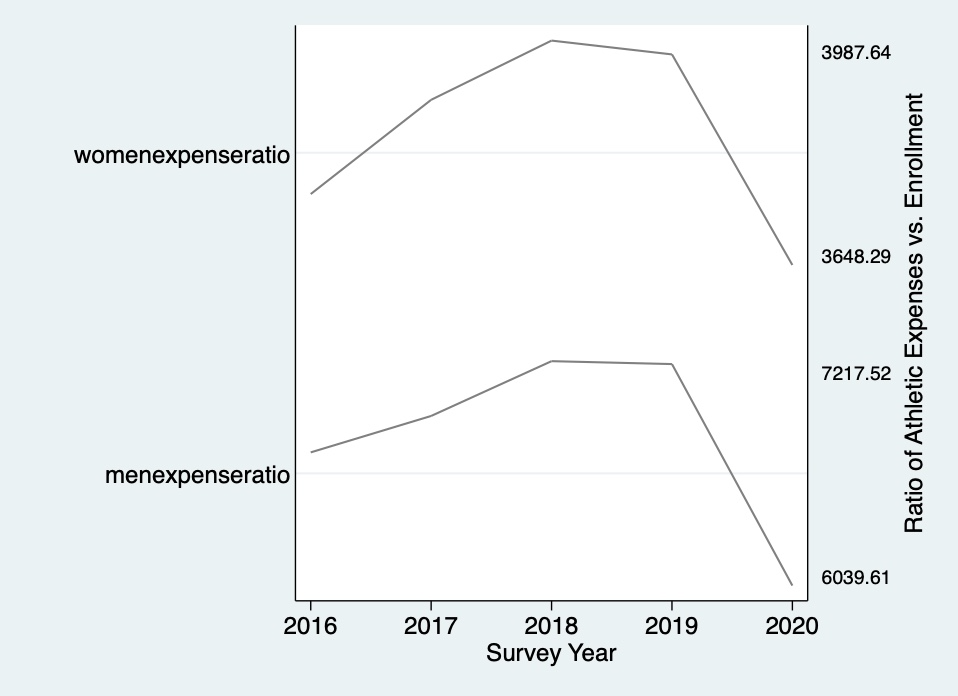
\includegraphics[scale = 0.75]{Graph.png}

The next step is to test if female expense: enrollment ratios are lower than male expense: enrollment ratios. This will be done with a paired t-test and the results are shown below. This shows that there is a significant difference between the male and female expenses where there is a gap of almost 3000 points between the male and female expenses, indicating that male teams received significantly more aid and funding over the five years under study.

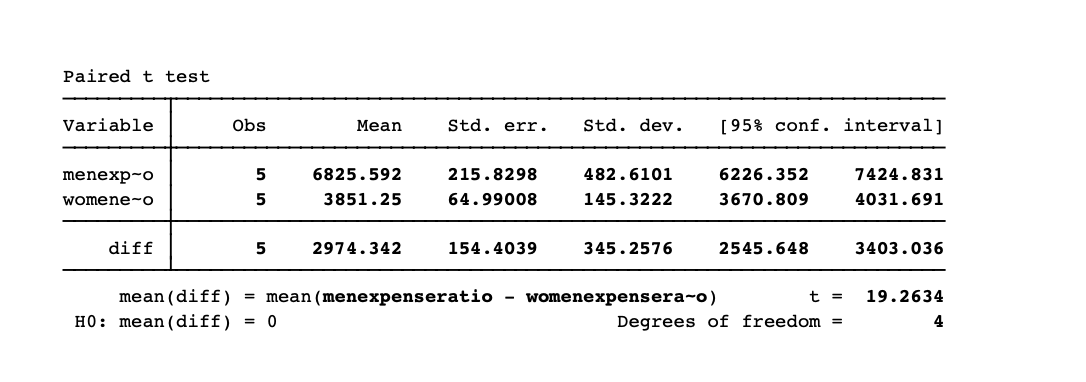
\includegraphics[scale = 0.75]{table.png}

This is at odds with the fact that female undergraduate enrollment has been consistently higher than male undergraduate enrollment in all eleven of these schools. A visual representation of this result is shown in the following graph. Here, it is clear that male enrollment has in fact dropped off since 2019 compared to female enrollment. This advances that there is a clear disparity in athletic funding for male and female teams given the decline in male and female enrollment over the past five years.

Further analysis on this topic will include a deep dive into each of the Big East schools and the discrepancies in between male and female athletic spending in each school and its associated programs. There is also potential to analyze coach compensation as an additional variable that speaks to the third prong of Title IX compliance: effectively accommodating interests and abilities. With expanded interest in athletics and with rising female enrollment, Title IX compliance includes providing avenues for improvement to female athletes in college teams through advanced guidance and coaches. Another potential variable of interest is recruiting expenses in the EADA dataset. It is assumed that to achieve substantial proportionality, schools are incentivized to reduce female interest in athletics so as to justify providing fewer services and aid to female athletic teams. Thus, if there is a significant decline in recruiting expenses for female athletic teams, scholars can judge if American universities are attempting to reduce opportunities to be judged as discriminatory.

\medskip

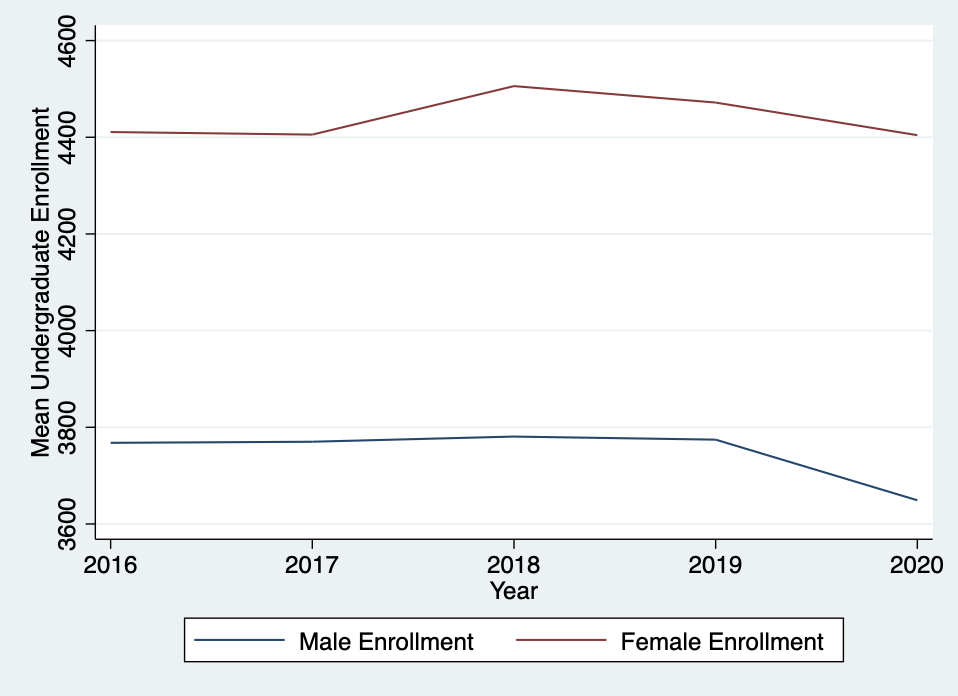
\includegraphics[scale = 0.75]{graph2.png}

\medskip

The significant gap between female and male athletic expenditure: enrollment ratio supports the initial hypothesis that there has been a decline in athletic aid and expenditure in the eleven Big East schools on average in the 2016 - 2020 period. This is specifically highlighted by declining male enrollment in these universities at the same time. These figures highlight possible Title IX compliance as measured by the first and third prongs, which stress substantial proportionality and effective accommodation of athletic interests respectively.

\section{Conclusion}
This research was inspired by a prominent lawsuit filed by the rowing team against the University of Connecticut in June 2020, when the court ruled that eliminating the rowing team due to pandemic-related budget cuts would violate Title IX. Future research could analyze trends in male-female athletic expenditure following periods of economic recessions and if there will be a drop in female athletic expenditure in the post-2008 and post-COVID pandemic periods. There are also possible avenues for research into the role that rising female university enrollment could play in leveling the playing field for women athletes as it is expected that expense: enrollment ratios are likely to decline further, and the disparities between male and female ratios will increase over time.

Title IX has opened up a door into studying sex-based discrimination in athletics and it remains as contested today as it was in 1972. Legal cases have been detailed the complicated terms of Title IX implementation, as the official definitions of substantial proportionality remain confusing. For example, the cases of \emph{Pederson v. LSU} \cite{Pederson}, \emph{Neal v. Board of Trustees of the California State Universities} \cite{Neal}, and \emph{Stanley v. the University of Southern California} \cite{Stanley} show that there are several considerations for legal adjudication of Title IX cases. \emph{Pederson} showed that there was Title IX compliance in Louisiana State University with 49\% female enrollment with only 29\% athletic participation. \emph{Neal}, on the other hand, showed the deleterious effects of reverse sexism in California State University when the court forced the university to comply with Title IX by reducing the number of men's wrestling scholarships, instead of improving the level of athletic participation in both genders. \emph{Stanley} was another important scenario when Marianne Stanley sued the University of South California for unequal pay as the women's basketball coach at USC. This reiterates another interesting application of this research by potentially using coach compensation for male and female sports teams as a proxy for providing effective athletic opportunities.

One of the biggest limitations of the study is that EADA numbers have been accused of not matching up to sports rosters as listed on school websites. Katie Thomas, a reporter for the \emph{New York Times}, wrote a series of articles in 2011 about how many NCAA Division I institutions like the Big East schools are padding their women's team rosters with underqualified athletes, and that universities have been undercounting their male athletes and over-counting their female athletes to make their participation gap look smaller \cite{Thomas}. This means that the EADA dataset used in this analysis might not be representative of real athletic numbers as reflected on the ground.

It is expected that this paper will contribute to an extended analysis of the Big East schools, and the role that a state flagship university like the University of Connecticut plays in upholding federal Title IX laws. Deeper research into drops in athletic expenditure in relation to national economic crises could reiterate interesting relationships between sports appetites and declining public fortunes. There are many possible research avenues to explore beyond this paper, but the ultimate goal is to continue to use rigorous research to shed light on institutional discrimination levied against female athletes.

\bibliographystyle{plain}
\bibliography{citations}
\end{document}